Ein adiabatischer Prozess beschreibt eine thermodynamische Zustandsänderung eines Systems, bei der kein Wärmeaustausch mit der Umgebung stattfindet. Eine wichtige Größe bei adiabatischen Prozessen ist der Adiabatenkoeffizient. In Versuch 221 werden zwei verschiedene Verfahren betrachtet, um den Adiabatenkoeffizienten zu bestimmen.

\subsection{Physikalische Grundlagen}

Eine adiabatische Zustandsänderung folgt der Gesetzmäßigkeit
\begin{align}
  p V^{\kappa} = \const \label{eq:adiabatisch}
\end{align}

Hierbei beschreibt $p$ den Druck im System, $V$ das Volumen des Systems und $\kappa$ den Adiabatenkoeffizient. Letzterer ergibt sich aus dem Verhältnis
\begin{align}
  \kappa = \frac{c_p}{c_V}
\end{align}
der spezifischen Wärmekapazität bei konstantem Druck $c_p$ und bei konstantem Volumen $c_V$.

Zur Bestimmung des Adiabatenkoeffizienten werden im folgenden Versuch zwei Verfahren betrachtet, das Verfahren nach Clément-Desormes und das Verfahren nach Rüchardt.

\subsubsection*{Bestimmung des Adiabatenkoeffizienten nach Clément und Desormes}

Der Aufbau nach Clément-Desormes ist in \abbref{fig:aufbau_cd} zu sehen.

\begin{figure}[H]
  \centering
  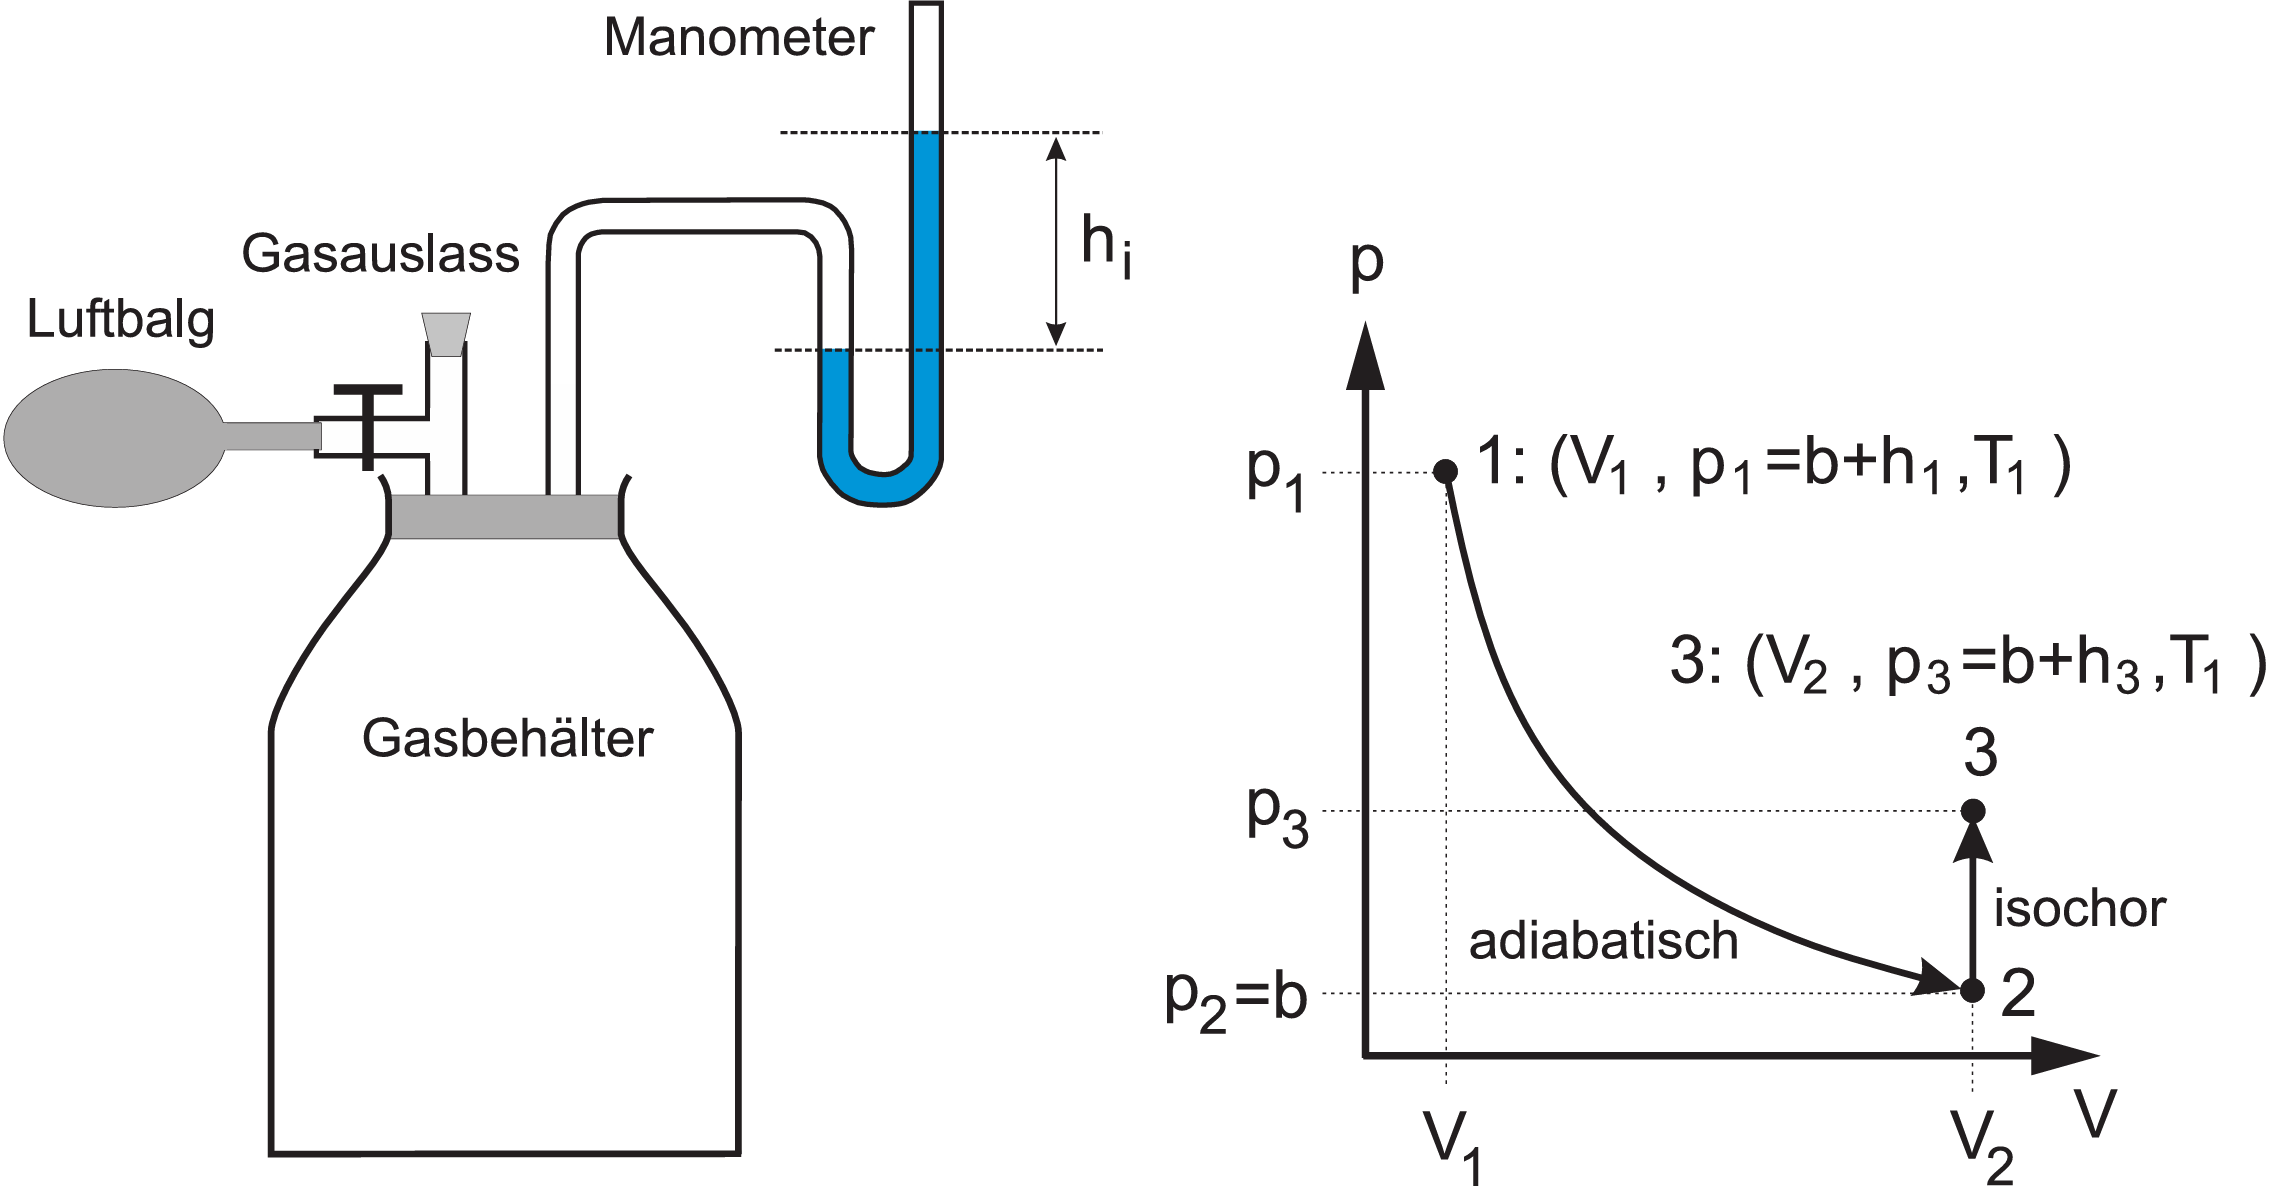
\includegraphics[width=0.8\textwidth]{files/aufbau_clement_desormes.png}
  \caption{Versuchsaufbau nach Clément-Desormes und zugehöriges $pV$-Diagramm}
  \label{fig:aufbau_cd}
\end{figure}

Dem nebenstehenden $pV$-Digramm sind die drei Zustände des Systems zu entnehmen, welche im Versuch betrachtet werden.

Erzeugt man durch pumpen des Luftbalgs einen Überdruck im System und lässt es daraufhin auf Zimmertemperatur abkühlen, so ist
\begin{align*}
  \text{\textbf{Zustand 1}: } V_1,\ p_1 = b + h_1,\ T_1
\end{align*}
mit Volumen $V_1$, äußerem Druck $b$, Höhendifferenz des Manometers $h_1$ und Temperatur $T_1$ (Zimmertemperatur) erreicht. Durch sehr kurzes öffnen des Gasauslasses erreicht man, optimalerweise ohne Wärmeaustausch mit der Umgebung, in einem adiabatischen Übergang den
\begin{align*}
  \text{\textbf{Zustand 2}: } V_2 = V_1 + \Delta V,\ p_1 = b,\ T_2 = T_1 - \Delta T.
\end{align*}
Die Volumenvergrößerung $\Delta V$ entspricht den im Prozess entwichenen Gasmolekülen. Während sich die Temperatur wieder an die Zimmertemperatur anpasst, erreicht man durch einen isochoren Übergang, also bei konstanten Volumen,
\begin{align*}
  \text{\textbf{Zustand 3}: } V_3 = V_2 = V_1 + \Delta V,\ p_1 = b + h_3,\ T_3 = T_1.
\end{align*}

Da die Zustandsänderung $1 \to 2$ adiabatisch abläuft, sind die beiden Zustände nach Gleichung \ref{eq:adiabatisch} verknüpft über die Poisson'sche Gleichung
\begin{align}
  p_1V_1^{\kappa} = p_2V_2^{\kappa}.
\end{align}
Nach dieser Beziehung berechnen wir mit
\begin{align}
  (b + h_1)V_1^{\kappa} &= b(V_1 + \Delta V)^{\kappa}
  \intertext{und der Näherung, dass $\Delta V \ll V_1$ die Gleichung}
  \frac{h_1}{b} &= \kappa \frac{\Delta V}{V_1} \label{eq:vol_rel_adiabat}.
\end{align}

Da die Temperaturen der Zustände 1 und 3 gleich sind, gilt nach dem Boyle-Mariott'schen Gesetz, dass
\begin{align}
  p_1 V_1 &= p_3 V_3
  \intertext{und somit}
  (b + h_1) V_1 &= (b + h_3) (V_1 + \Delta V).
  \intertext{Mit den Näherungen $\Delta V \ll V_1$ und $\Delta h_3 \ll b$ erhalten wir daraus}
  \frac{\Delta V}{V_1} &= \frac{h_1 - h_3}{b}.
\end{align}
Gemeinsam mit Gleichung \ref{eq:vol_rel_adiabat} erhalten wir die Gleichung
\begin{align}
  \kappa = \frac{h_1}{h_1 - h_3} \label{eq:adiabat_nach_cd}
\end{align}
für den Adiabatenkoeffizienten.

\subsubsection*{Bestimmung des Adiabatenkoeffizienten nach Rüchardt}

Bei der Bestimmung nach Rüchardt betrachten wir einen Schwingkörper welcher in einem Glasrohr durch adiabatische Expansion und Kompression in Schwingung versetzt wird. Als Gleichgewichtssituation betrachten wir die Summe aus Luftdruck $p_0$ und Schweredruck $\frac{mg}{A}$ des Schwingkörpers
\begin{align}
  p = p_0 + \frac{mg}{A}.\label{eq:pressure_sum}
\end{align}
Für eine infinitesimale Schwingung des Körpers gilt nach dem ersten Newton'schen Gesetz
\begin{align}
m \dv[2]{x}{t} = A \dd{p} \label{eq:durck_osz}.
\end{align}

Da der Prozess adiabatisch abläuft, gilt Gleichung (\ref{eq:adiabatisch}). Durch das Ableiten dieser nach $p$ erhalten wir den Zusammenhang
\begin{align}
  \dd{p} = -\kappa \frac{p}{V} \dd{V}.
\end{align}
Eingesetzt in \ref{eq:durck_osz} erhalten wir daraus
\begin{align}
  m \dv[2]{x}{t} = - A \kappa \frac{p}{V} \dd{V}.
\end{align}
Identifizieren wir zusätzlich die Volumenänderung $\dd{V}$ mit der Bewegung des Schwingkörpers $\dd{V} = A x = \pi r^2 x$, so erhalten wir die Bewegungsgleichung eines harmonischen Oszillators
\begin{align}
  \ddot{x} + \frac{\pi^2 r^2 \kappa p}{m V} x = 0.
  \intertext{Daraus lesen wir die Kreisfrequenz und die Periodendauer}
  \omega = \sqrt{\frac{\pi^2 r^2 \kappa p}{m V}},\quad  T = \sqrt{\frac{4mV}{r^4 \kappa p}}
\end{align}
ab. Damit haben wir einen weiteren mathematischen Zusammenhang für den Adiabatenkoeffizienten hergeleitet:
\begin{align}
  \kappa = \frac{4 m V}{r^4 T^2 p} \label{eq:kappa_ruchart}.
\end{align}

\subsection{Versuchsdurchführung}

Wir begannen die Versuchsdurchführung mit der Messung nach Rüchardt und führten diese für Druckluft und Argon durch. Im zweiten Teil führten wir die Messung nach Clément-Desormes für Luft durch.

\textbf{Messung nach Rüchardt.} Für sowohl Druckluft, als auch Argon, nahmen wir zunächst den Umgebungsluftdruck und die Maße des Versuchsaufbaus auf. Danach nahmen wir in jeweils drei Messgängen die Zeit für 50 Schwingungen auf.

\textbf{Messung nach Clément-Desormes.} Die notwendigen Schritte der Durchführung (Pumpen, Temperatur angleichen lassen, Pfropfen öffnen) sind bereits in den theoretischen Grundlagen genannt. Für fünf Durchgänge nahmen wir die Höhen $h_1$ und $h_3$ vom Manometer ab.